\section{Principles of Serial Communication \embsys{475}{9}}
\vspace{-.5cm}
\begin{multicols}{2}
    \begin{minipage}{\linewidth}
	\textbf{Baud-Rate (BR)}
    \[\frac{1}{t_{symbol}}=Baudrate [bd]\]
	Expresses the number of symbols per second. If one bit per symbol then bitrate is equal to baudrate. Often 2 Bits per symbol or more then bitrate is higher than baudrate.\\ 
    \end{minipage}

    \begin{minipage}{\linewidth}
	\textbf{Bitrate}
    \[\frac{1}{t_{bit}}=Bitrate [bit/s]\]
	Expresses the number of bits-per-second transmitted in the channel. \\
    \end{minipage}
\end{multicols}
\vspace{-1cm}
\subsection{Data Communication Fundamentals \embsys{475}{9.1}}
	\subsubsection{Serial Data Channels}
	\begin{itemize}
		\item RX: Receiver, TX:Transmitter
		\item Main form of Communications today
		\item Broad variaton of Protocols and Formats
		\item Bits are transmitted and received one after another
		\item longer time for sending bits $n\cdot t_{bit}$
		\item Single Ended Link: Two Wires (Link, \acs{GND})
		\item Differential Link Channel: Two Wires with Voltage Difference
		\item \acs{USB}, RS232, RS485, Bluetooth, Ethernet, \acs{I2C}, \acs{SATA}...
	\end{itemize}
\subsubsection{Parallel Data Channels}
	\begin{itemize}
		\item n Bits are transferred simultaneously in parallel
		\item needs a wire for every bit $ \rightarrow $ expensiv!
	\end{itemize}
	
\subsection{Types of Serial Channels \embsys{477}{9.2}}
\subsubsection{Type of Connectivity}
\begin{tabular}{lll}
	\textbf{Simplex}&\textbf{Half-Duplex} &\textbf{Duplex}\\
	Unidirectional Link&  One Bidirectional Link& Two separate Bidirectional Link\\
	Only one Direction & both Directions & both Directions\\
	No \acs{ACK} of Data & one Direction at one Time & Simultaneous Communication\\
	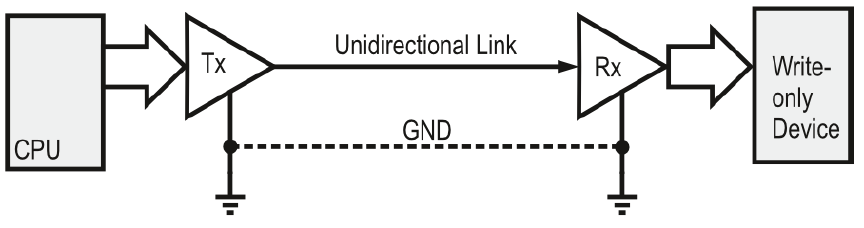
\includegraphics[width=6cm]{images/simplex.png}& 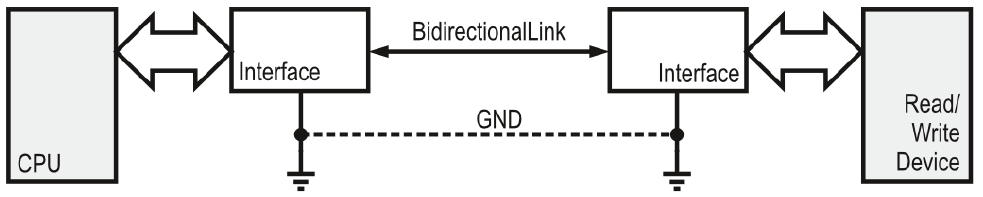
\includegraphics[width=6cm]{images/half_duplex.png}&
	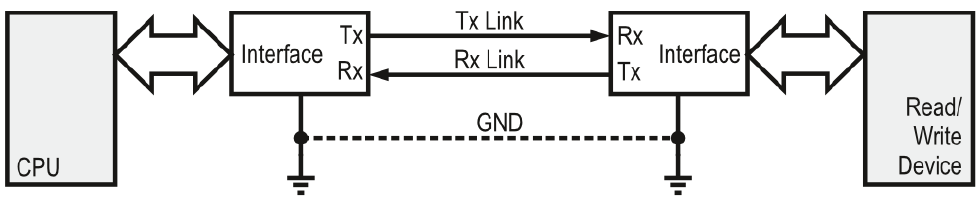
\includegraphics[width=6cm]{images/duplex.png}\\
\end{tabular}
\begin{minipage}{0.2\linewidth}
	\subsubsection{Topologies}
	\begin{itemize}
		\item Point-to-Point
		\item Bus
		\item Line
		\item Star
		\item Ring
	\end{itemize}
\end{minipage}
\begin{minipage}{0.8\linewidth}
	\subsubsection{Signaling}
	\begin{itemize}
		\item Single-ended signaling (asymmetrischer Signalübertragung)
		\subitem One wire carries a varying voltage, the other wire a reference voltage
		\item Differential Signaling (symmetrischer Signalübertragung)
		\subitem Receiving circuit responds to the electrical difference between the two signals
	\end{itemize}
\end{minipage}
	
\clearpage
\pagebreak
\subsection{Asynchronous Serial Communication \embsys{479}{9.3.1}}
\begin{minipage}{12cm}
	\begin{itemize}
		\item Asynchronous Channels: Independent Clock at both Ends	
		\item Clocks must be synchronized regularly
		\item Each Package contains of Header (begin Data), Body (Data), Footer (delimits the Packet)
		\item Same Data rate at both Ends
		\item Falling Edge of Startbit starts Sampling at RX
		\item Receiver Samples in the middle of each Bit
		\item If RX runs too fast then ends in incorrect Datagram
		\item Bad Rate Erros of $2\%$ to $4\%$ are tolerable
	\end{itemize}
\end{minipage}
\begin{minipage}{7cm}
	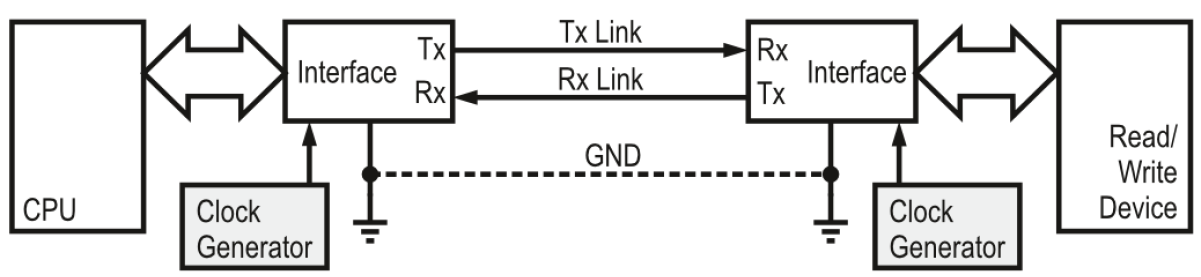
\includegraphics[width=7cm]{images/asyn.png}
\end{minipage}

\subsubsection{Error Detection Mechanism}
\begin{itemize}
	\item Even Parity: If the number of "'1"' is even (gerade) in the bit string then the paritybit is even \newline If for the data communciation even parity given then paritybit is "'0"' for even and "'1"' for odd. 
	\item Odd Parity: If the number of "'1"' is odd (ungerade)in the bit string then the paritybit is odd \newline If for the data communciation odd parity given then paritybit is "'1"' for even and "'0"' for odd.
	\item Parity Bit: can be configured to Even, Odd, None, Mark, Space
	\item Stop Bit: marks the End of the Transmission, always Mark
\end{itemize}
\subsubsection{Universal Asynchronous Receiver Transmitter (\acs{UART})}
\begin{minipage}{10cm}
	\begin{itemize}
		\item convert Data from Parallel to Serial and viceversa
		\item allow the \acs{CPU} to communicate through the Serial Channel
		\item Logic Levels, Positive Logic Level (1=high, 0=low)
		\item \acs{USART}: Asynchronous and Synchronous Communications Channels in one single Serial Interface Module
		\item Choosing the clock source $N=\frac{f_{clk}}{BR}$
		\item Configuring the baud rate generator
		\item Choosing and configuring parity check, stop bit length
		\item \textbf{\acs{DSR}: }Data Set is Ready
		\item \textbf{\acs{DTR}: }Data Terminal is Ready
		\item \textbf{\acs{RTS}: }Request to Send
		\item \textbf{\acs{CTS}: }Clear to Send
		\item \textbf{\acs{TxD}: }Transmitted Data
		\item \textbf{\acs{RxD}: }Received Data
	\end{itemize}
\end{minipage}
\begin{minipage}{9cm}
	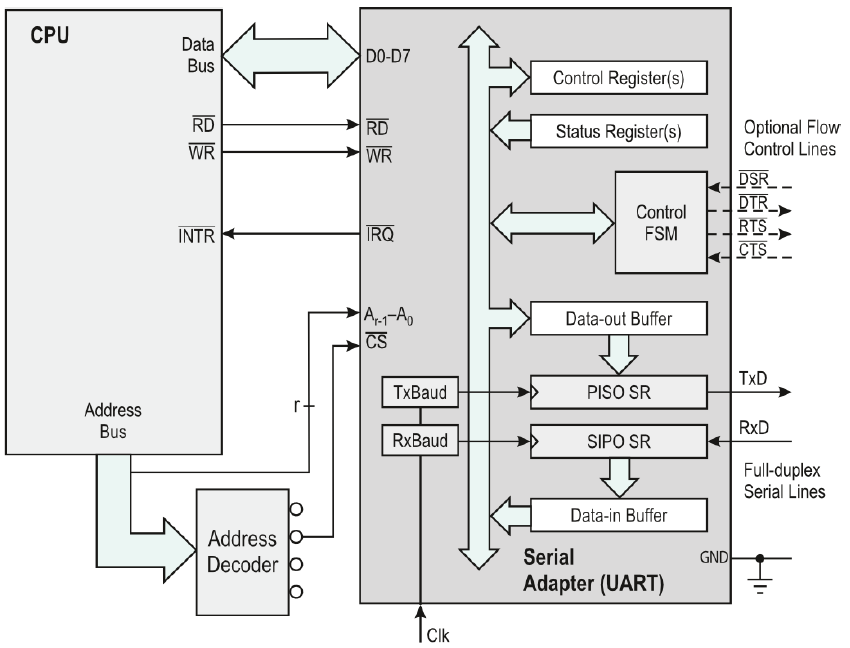
\includegraphics[width=9cm]{images/uart.png}
\end{minipage}

\subsubsection{RS-232}
\begin{minipage}{10cm}
	\begin{itemize}
		\item asynchrone and Point to Point Link
		\item One symbol consist of 5 to 9 Bit, often \acs{ASCII}-Code (7 or 8 Bit per Symbol)
		\item Physical Voltages, Negative Logic
		\item $1=-25V \quad to \quad -3V$\newline
		$0=+25V\quad to \quad +3V$
		\item Long history in Telephone-Modem Applications
		\item Connectors DB-25 (D-Sub 25 Pin) and DB-9 (D-Sub 9 Pin)
		\item\textbf{RI: }Ring Indicator, signals an incoming call
	\end{itemize}
\end{minipage}
\begin{minipage}{6cm}
	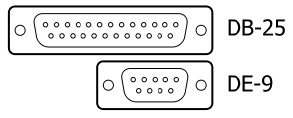
\includegraphics[width=6cm]{images/Connectors_RS.png}
\end{minipage}
\\
\begin{tabular}{ccc}
	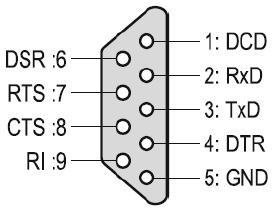
\includegraphics[width=4cm]{images/pin_RS.png} & 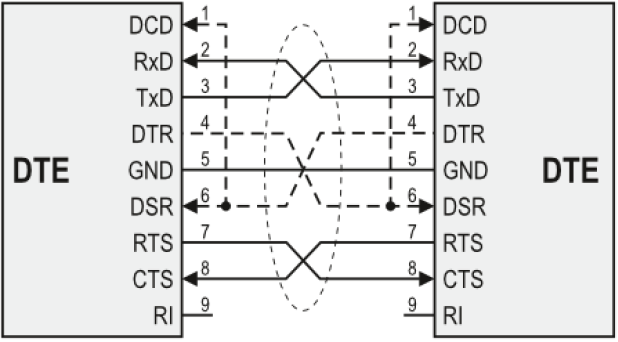
\includegraphics[width=6cm]{images/cable2_RS.png} & 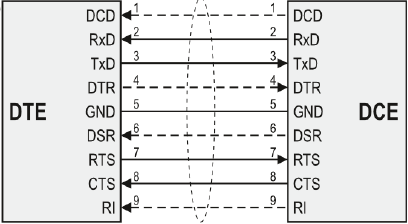
\includegraphics[width=6cm]{images/cable_RS.png}\\
\end{tabular}
\begin{multicols}{2}
    \subsubsection{RS-422}
    \begin{itemize}
    	\item Duplex, symmetric Bus
    	\item One driver an ten Receivers
    	\item Differential Serial Link
    \end{itemize}
    \subsubsection{RS-485}
    \begin{itemize}
    	\item Bidirectional, Halfduplex Bus
    	\item allows 32 Drivers and 32 Receiver in a single Bus topology
    	\item Termination Impedance $120 \Omega$
    \end{itemize}
\end{multicols}

\subsubsection{Universal Serial Bus (\acs{USB})}
\begin{multicols}{2}
	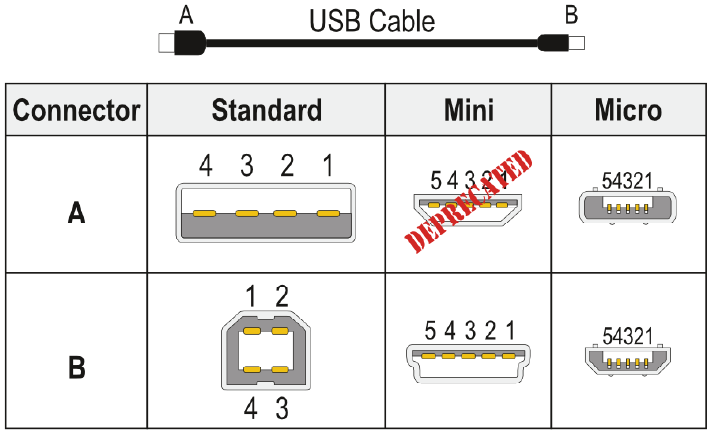
\includegraphics[width=8cm]{images/usb_jacks.png}\\
	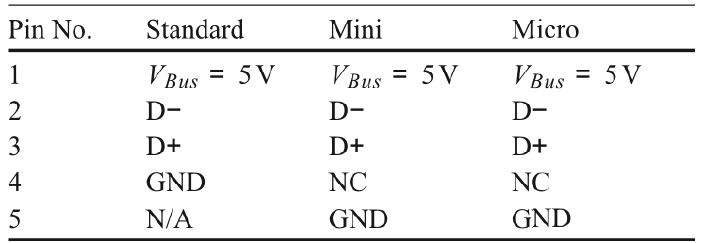
\includegraphics[width=8cm]{images/usb_voltage.png}\\
\end{multicols}

\begin{minipage}{12cm}
    \subsection{Cirular Buffer}
    CodeBSP siehe Anhang \label{CircularBuffer}
	\begin{itemize}
		\item UART Hardware do sends/receive information in a sequence of Bytes
		\item After Transmission/Reception (Tx/Rx) of each Byte, UART-states are monitored in dedicated Flags
		\item User Application shall be decoupled from sending/receiving Data
	\end{itemize}
\end{minipage}
\begin{minipage}{5cm}
	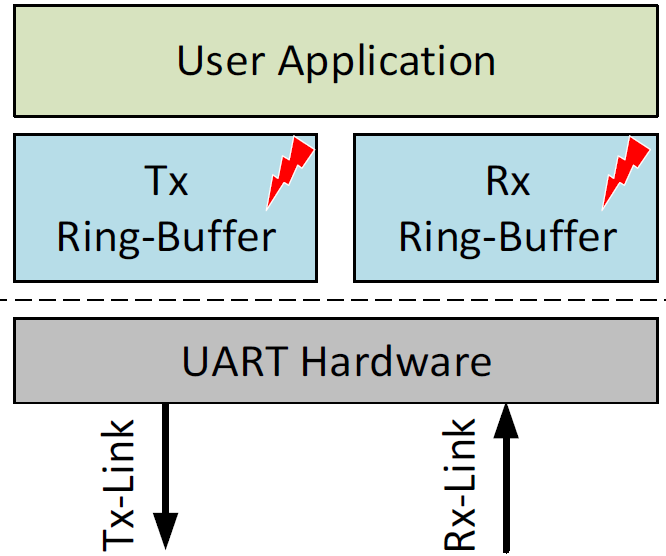
\includegraphics[width=5cm]{images/ringbuffer.png}
\end{minipage}
\begin{multicols}{2}
\subsubsection{RX Implementation}
When Bytes are received Rx \acs{ISR} reads the Byte from the \acs{UART} in Rx-Ring-Buffer and places data in Ringbuffer. \\
The User Application reads received Byte from the Rx-Ring-Buffer. The "oldest" Byte (least recent Byte) is extracted first from the Rx-Ring-Buffer.\\
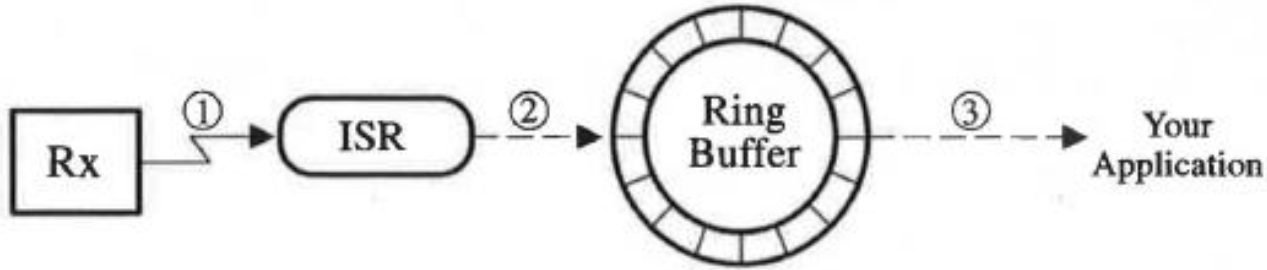
\includegraphics[width=8cm]{images/rx_buffer.png}
\subsubsection{TX Implementation}
When Bytes need to be sent Bytes are placed into the Tx-Ring-Buffer Tx \acs{ISR} are enabled after putting a Byte into the Tx-Ring-Buffer. \\
If the UART is ready to send a Byte an TX Interrupt occurs and the ISR extracts the "oldest" (least recent) Byte from the Tx-Ring-Buffer. The byte is then output to the UART.\\
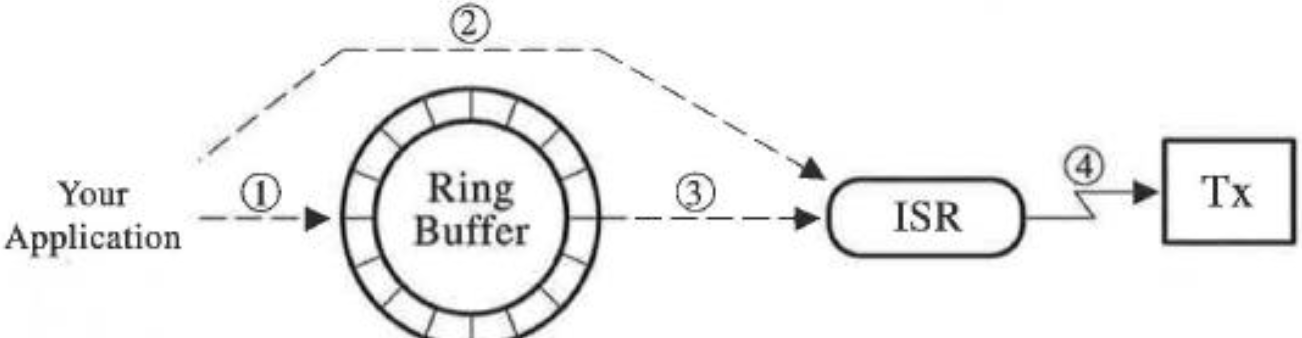
\includegraphics[width=8cm]{images/tx_buffer.png}
\end{multicols}
\clearpage

\subsubsection{Flow Control}
To avoid allocating very large buffers, flow control can be introduced.
The Receiver can notify the remote sender that the receiver's buffer is getting full.
The remote sender would then hold off with its transmission until the receiver empties out the buffer and notifies the sender that it can proceed.
For this concept there are two implementations:
\begin{itemize}
	\item \textbf{XON-XOFF} uses \acs{ASCII} characters
	\subitem DC1 (0x11) for XON, send more data
	\subitem DC3 (0x13) for XOFF, don't send more
	\item \textbf{RS-232} use lines of RS-232
	\subitem \acs{RTS}, \acs{CTS}, \acs{DSR}, \acs{DTR} allowing to send data
\end{itemize}
\subsection{Synchronous Serial Communication \embsys{498}{9.4}}
\begin{minipage}{11cm}
	\begin{itemize}
		\item Both transmitting and receiving data are with the same Clock Signal
		\item Data and Clock Signal are transmitted over the channel
		\item Usually Master/Slave-Mode
		\item Datagrams can be longer than those in asynchron
		\item Multidrop possible
	\end{itemize}
\end{minipage}
\begin{minipage}{8cm}
	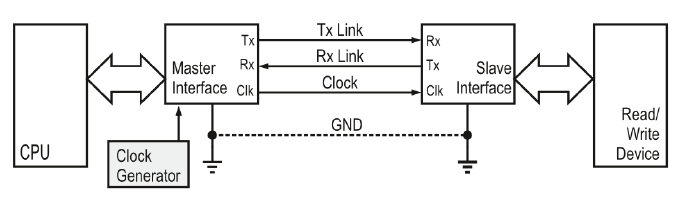
\includegraphics[width=8cm]{images/syn.png}
\end{minipage}
%=========================================================================
%\clearpage
%\pagebreak
\subsubsection{Serial Peripheral Interface Bus (\acs{SPI})} 
\begin{multicols}{2}
    \begin{itemize}
    	\item Fullduplex
    	\item defines the relay of Packets between a Master and one or more Slaves only (Physical Layer of Communication)
    	\item does not specify any Data, Session, or higher-level Protocol
    	\item single Shift Register that serves as both, Receiver and Transmitter, synchronized by the Transmission Clock
    	\item limited interfaced Distance
    	\item no Error Checking Mechanism
    	\item Each Slave contain a \acs{MISO} Driver which is activatet by the \acs{SS}-Line
    	\item Chained Configuration: Slaves share \acs{SS} and between slave \acs{MISO}, \acs{MOSI} are connected
    	\item Four Clock modes are available
    	\item \acs{SS}: select Slave, activate \acs{MISO} and signalize Start and End of Data
    \end{itemize}
\end{multicols}
\begin{minipage}{0.6\linewidth}
    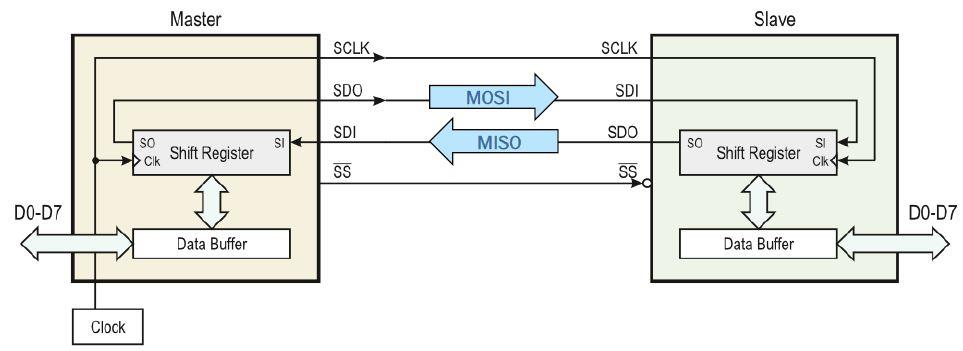
\includegraphics[width=\linewidth]{images/spi.png}
\end{minipage}
\begin{minipage}{0.4\linewidth}
     \textbf{Data Transfer}
    \begin{enumerate}
    	\item Store Data into Data Buffer, copied into Shift Register
    	\item Activate Slave Select
    	\item Common-Clocked Data-Transfer between Shift Registers
    	\item Deactivate Slave Select
    	\item Copied received Date into Data Buffer, Read Data
    \end{enumerate}
\end{minipage}
%=========================================================================
\clearpage
%\pagebreak
\vspace{-1cm}
\subsubsection{Inter-Integrated Circuit Bus ($I^2C$)}
\begin{minipage}{13cm}
	\begin{itemize}
		\item Typical Speed 100kbps, 400kbps
		\item Maximal 127 slave addressable
		\item Board Level Interconnection of IC Modules
		\item Halfduplex, Multidrop Bus, bidirektional
		\item Bus Length is expected short and limited to PCB-Level
		\item Low-State is always dominant over High-State
		\item \acs{I2C}-Hardware provides Start/Stop, Clock Synch, Clock stretching, Bus Arbitration
		\item Multi-Master Capability with Collision Detection and Arbitration Mechanisms
		\item \textbf{\acs{SDA}: }Serial Data
		\item \textbf{\acs{SCL}: }Serial Clock
	\end{itemize}
\end{minipage}
\begin{minipage}{6cm}
	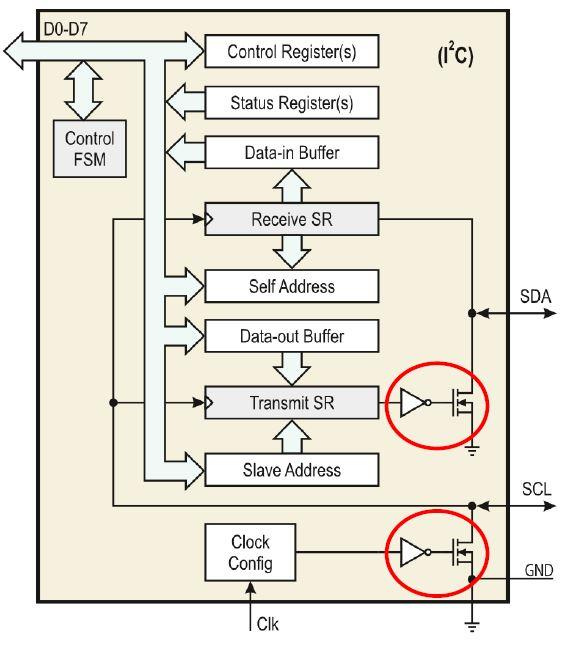
\includegraphics[width=6cm]{images/i2c_internal.png}
\end{minipage}
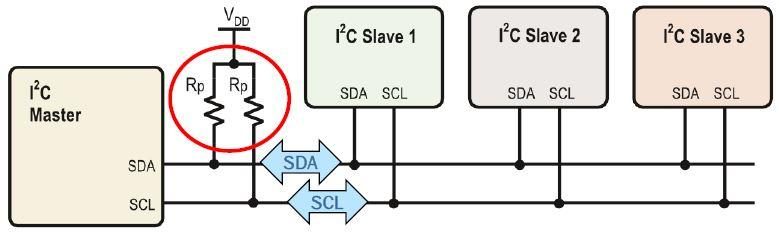
\includegraphics[width=12cm]{images/i2c_1.png}
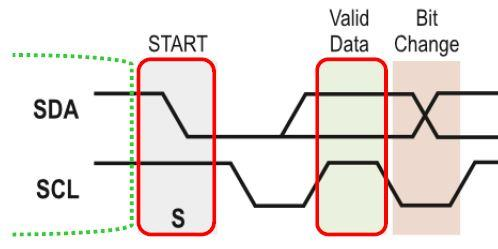
\includegraphics[width=6cm]{images/i2c_2.png}\\
\begin{minipage}{\linewidth}
	\begin{itemize}
		\item Protocol contains three different conditions
		\subitem Start condition (S) : Master takes Control and initiates a Transfer
		\subitem Data Transfer: \acs{SCL} with low-high, \acs{SDA} changed only when SCL=low
		\subitem Stop condition (P): closes a Transfer
		\subitem Idle State
		\item Arbitration Process determines which Master will remain in Control
		\subitem Masters who place a Logic High-Level conflict with the Low-Level Data placed by another Master and loss Control of the \acs{I2C}-Bus
		\subitem The Master who addresses the Slave with the lowest Address wins the Arbitration Race
	\end{itemize}
\end{minipage}

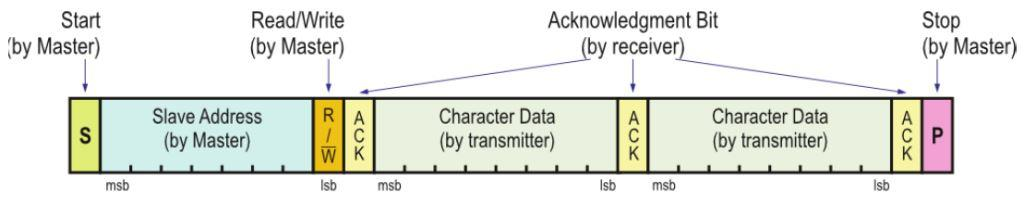
\includegraphics[width=16cm]{images/i2c_data.png}\\
%=========================================================================


\subsubsection{MSP430 Serials Components}
\begin{tabular}{ll}
    \acs{USART} &
    provide \acs{UART} and \acs{SPI} connectivity\\
    
    \acs{SCI} &
	Serial Communication Interface modules that provide fundamental \acs{SPI} and \acs{I2C} capabilities.\\
    
	\acs{USI} &
	Universal Serial Interface, simplest Serial Interface support only \acs{SPI} and \acs{I2C}\\
    
	\acs{USCI} &
	Universal Serial Communication Interface, with wide support for \acs{UART}, \acs{SPI}, and \acs{I2C} modes.\\
    
	\acs{USB} & Universal Serial Bus\\
    
\end{tabular}
\clearpage
\pagebreak
